\documentclass[12pt, twoside]{article}
\usepackage{jmlda}
\newcommand{\hdir}{.}


\begin{document}

\title
    {Распознавание текста на основе скелетного представления толстых линий и сверточных сетей}
\author
    {А.\,С.~Лукоянов$^1$} 
\email
    {lukoyanov.as@phystech.edu}
\thanks
    {Работа выполнена при
     %частичной
     финансовой поддержке РФФИ, проекты \No\ \No 00-00-00000 и 00-00-00001.}
\organization
    {$^1$МФТИ}
    
\abstract{
\noindent
\textbf{Аннотация}: Данная работа посвящена решению задачи оптического распознавания символов при помощи скелетного представления. Такой подход имеет несколько недостатков, один из них заключается в неприменимости традиционных сверточных нейронных сетей на графовых структурах, которые и являются результатом склетизации символов. В данной работе мы предлагаем способ свертывания графовых структур, позволяющий породить информативное описание скелета толстой линии. Также приводится сравнительный анализ архитектур, работающих непосредственно на растровом представлении символов и  архитектур, использующих графовое представление символов.  Для этих целей используется классический в подобных задачах набор данных MNIST, на котором нам удалось добиться значимого повышения качества распознавания толстых линий за счет нового способа порождения их описаний.
	
\bigskip
\noindent
\textbf{Ключевые слова}: \emph {классификация символов; распознование текста; графовые структуры; скелетное представление; свертки.}
}

%данные поля заполняются редакцией журнала
\doi{10.21469/22233792}
\receivedRus{01.01.2017}
\receivedEng{January 01, 2017}

\maketitle
\linenumbers
\section{Введение}
Задача оптического распознования символов уже стала классической среди задач компьютерного зрения. Несмотря на то, что качество существующих моделей довольно высоко, каждый год выходит множество научных работ, посвященных именно класификации символов~\cite{MNIST_capsule}~\cite{MNIST_dl}. Основным подходом к решению таких задач стали архитектуры, использующие сверточные слои~\cite{cnn_lecun}~\cite{cnn_appl}. Традиционно, входом таких алгоритмов является растровое изображение, но, тем не менее, существует более комплексный подход, при котором растровое изображение сначала переводится в векторное представление путем построения скелета сивола, то есть графовой структуры, а потом подается на вход обучаемой модели. 

Наиболее общий подход к скелетизации представляет собой процесс заполнения внутренностей символов кругами, центры которых - будущие вершины графа, соединяются будущими ребрами графа. Например, в работе~\cite{graphs_gen} обсуждается моделирование рукописного текста с помощью жирных линий. В работе~\cite{graphs_shape_comp} проводится сравнение формы бинарных растровых изображений на основе скелетизации. Однако, существует и альтернативные методы, как, например описанный в работе~\cite{graphs_alt_method}. 

При этом, применение сверточных нейронных сетей на векторном представлении изображений является нетривиальной задачей, в следствии того, что традиционные методы сверток неприменимы для таких структур данных. 

Среди задач оптического распознавания символов и задач компьютерного зрения в целом особое место занимает задача классификации рукописного текста MNIST~\cite{mnist_original}. Большое количество работ, в том числе и современных, используют данную выборку для валидации и сравнения предложенных архитектур, как в работах~\cite{mnist_sample1}~\cite{mnist_sample2}. Например, в докладе~\cite{mnist_sample3} рассматривается многозадачное обучение на данных MNIST.


\section{Постановка задачи}

Введем следующие обозначения: 
\begin{itemize}
\item $\mathbb{I}$ - множество бинарных изображений символов из алфавита $\mathbb{A}$. На изображении содержится только один символ и площадь описанной вокруг него окружности близка к площади окружности вписанной в квадрат изображения. При этом считаем, что для каждого элемента из $\mathbb{I}$ известна метка класса $y \in \mathbb{A}$. 

Тогда, пусть функция $a: \mathbb{I} \rightarrow \mathbb{A}$ однозначно сопоставляет каждому изображению из $\mathbb{I}$ его метку класса.

\item $\mathbb{G}$ - множество скелетных представлений изображений, где под скелетным представлением подразумевается неориентированный граф, каждой вершине которого сопоставлено некоторое число, называемое радиусом.

Функция $g: \mathbb{I} \rightarrow \mathbb{G}$ однозначно сопоставляет каждому изображению из $\mathbb{I}$ его скелетное представление. В данной работе в качестве такой функции используется алгоритм, описанный в работе~\cite{graphs_gen}.

\item $\mathbb{F}$ - множество признаков, описывающих скелетное представление символов. Получение конкретного вида этих признаков является одной из задач данной работы.

Функция $f: \mathbb{I} \rightarrow \mathbb{G}$ однозначно сопоставляет каждому элементу из $\mathbb{G}$ множество его признаков.
\end{itemize}

Тогда, задачей данной работы, является построение таких функций
 $$\hat{a_1}: \mathbb{I} \rightarrow \mathbb{A}$$
 $$ \hat{a_2}: \mathbb{G} \rightarrow \mathbb{A} $$ 
 $$\hat{a_3}: \mathbb{F} \rightarrow \mathbb{A}$$
 , что они минимизируют соответствующие функции потерь:
 $$L(\hat{a_1}, a)$$
 $$L(\hat{a_2}(g), a)$$ 
 $$L(\hat{a_3}(f(g)), a)$$
 , где $L(a, b)$ - функция кросс энтропии двух функций a и b на выборке изображений $\mathbb{I}$.
 
 
 \section{Описание эксперимента}
 Выполненная работа состоит из нескольких частей, каждую из которых рассмотрим подробнее:
 \begin{enumerate}
 \item \textbf{Обучение базовой модели, ставшей классической для задачи распознавания символов.}
 
 В качестве базовой модели было решено выбрать классическую модель VGG-16  << Доделать эксперимент и описать качество>>
  
 \item \textbf{Построение модели, приближающей функцию $ \hat{a_2} $.}
 
 В процессе построения такой модели возник ряд сложностей. Одной из них стало то, что графовое описание имеет нефиксированный размер, что приводит к невозможности обучения модели непосредственно на скелетизированном изображении. 
 
Для того чтобы решить эту проблему мы составили статистические признаки, которые в общем случае не зависят от количества ребер и вершин в графе. Статистические признаки, которые мы использовали в данной роботе это наименьшее, наибольшее, среднее значение и стандартное отклонение вычисленные на распределении каждой из следующих сущностей:
 
 \begin{itemize}
 \item Координата X каждого ребра, представленного в виде вектора.
 \item Координата Y каждого ребра, представленного в виде вектора.
 \item Угол наклона каждого ребра.
 \item Длина каждого ребра.
 \item Координата X каждой вершины.
 \item Координата Y каждой вершины.
 \item Радиус каждой вершины.
 \end{itemize}
 
 Так же, помимо описанных выше признаков, было добавлено количество вершин и гистограмма направлений. Под гистограммой направлений подразумевается 10 целых чисел, каждому из которых сопоставлен один из 10 равных секторов, разделяющих окружность. Каждое число отображает количество векторов, направленных в данный сектор.
 
Итого, таким образом было получено 39 признаков. В качестве модели был выбран градиентный бустинг над решающими деревьями, а именно Lightgbm. Для оптимизации гипер-параметров быд запущен grid-search, в результате чего точность (accuracy) составила 93,80%.
 
 
 \item  \textbf{Анализ ошибок.}
 Важной частью исследования является анализ ошибок. Получив, описанную выше модель и перебрав гипер-параметры, мы изучили примеры изображений, на которых полученная модель дает неверный результат. В подавляющем большинстве случаев, на этих изображениях граф скелетного представления недостаточно хорошо приближал нарисованную цифру. Связано это было с тем, что некоторые цифры содержат слишком тонкие или короткие участки, на которых алгоритм склетизации не способен построить адекватное приближение графом. Пример можно увидеть на изображении~\ref{fig:bad_sample}. В следствии этого был сделан вывод, что для дальнейшего улучшения качества системы, требуется более тонкая подстройка алгоритма скелетизации.
 
 \begin{figure}[H]
	\begin{center}
 		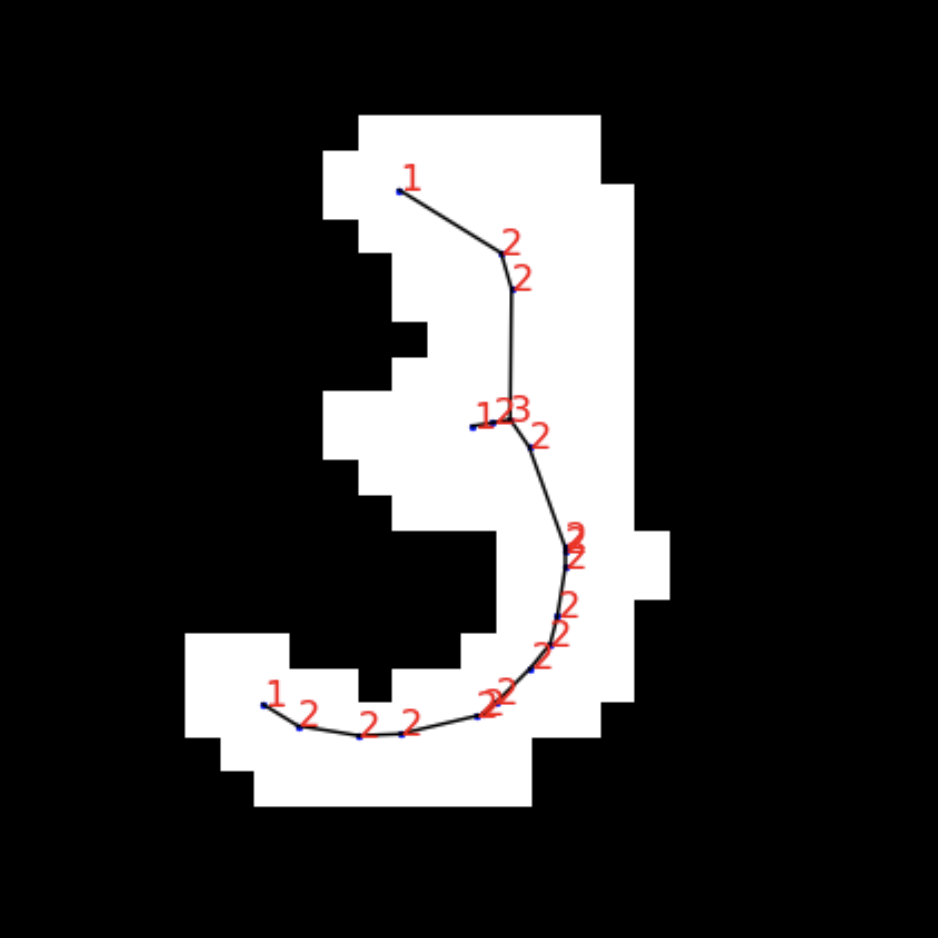
\includegraphics[width=0.6\textwidth]{bad_sample.jpg}
 	\end{center}
  \caption{Пример некорректной скелетизации}
  \label{fig:bad_sample}
\end{figure}

 \end{enumerate}

\begin{thebibliography}{1}
\bibitem{MNIST_capsule}
	\BibAuthor{Zou, Xianli}
	Fast Convergent Capsule Network with Applications in MNIST"---
	Advances in Neural Networks -- ISNN 2018"---
	Springer International Publishing"---
	pp. 3--10

\bibitem{MNIST_dl}
	\BibAuthor{Palvanov A., Im Cho Y}
	Comparisons of deep learning algorithms for MNIST in real-time environment"---
	International Journal of Fuzzy Logic and Intelligent Systems"--- 2018. – Т. 18. – №. 2. – С. 126-134.
	
\bibitem{cnn_lecun}
	\BibAuthor{LeCun Y. et al.}
	 Convolutional networks for images, speech, and time series //The handbook of brain theory and neural networks. – 1995. – Т. 3361. – №. 10. – С. 1995.
	 
\bibitem{cnn_appl}
	\BibAuthor{Ciresan D. C. et al.}
 	Convolutional neural network committees for handwritten character classification //Document Analysis and Recognition (ICDAR), 2011 International Conference on. – IEEE, 2011. – С. 1135-1139.
 
\bibitem{graphs_gen}
	\BibAuthor{Клименко С. В., Местецкий Л. М., Семенов А. Б.}
	 Моделирование рукописного шрифта с помощью жирных линий //Труды. – 2006. – Т. 16.

\bibitem{graphs_shape_comp}
	\BibAuthor{Кушнир О. и др.}
	 Сравнение формы бинарных растровых изображений на основе скелетизации //Машинное обучение и анализ данных. – 2012. – Т. 1. – №. 3. – С. 255-263.
	 
\bibitem{graphs_alt_method}
	\BibAuthor{Масалович А., Местецкий Л.}
	 Распрямление текстовых строк на основе непрерывного гранично-скелетного представления изображений //Труды Международной конференции «Графикон», Новосибирск.–2006.–4 c.

\bibitem{mnist_original}
	\BibAuthor{LeCun Y., Cortes C., Burges C. J.}
	MNIST handwritten digit database //
	Available: 
	 \BibUrl{http://yann. lecun. com/exdb/mnist}. – 2010. – Т. 2.

\bibitem{mnist_sample1}
	\BibAuthor{Zhu D. et al.}
	 Negative Log Likelihood Ratio Loss for Deep Neural Network Classification //arXiv preprint arXiv:1804.10690. – 2018.
	 
\bibitem{mnist_sample2}
	\BibAuthor{Nair P., Doshi R., Keselj S.}
	Pushing the limits of capsule networks //Technical note. – 2018.

\bibitem{mnist_sample3}
	\BibAuthor{Hsieh P. C., Chen C. P.}
	 Multi-task Learning on MNIST Image Datasets. – 2018.

\end{thebibliography}

\end{document}
